\chapter{Labeled SCC Filter}
\label{chap:lsf}

\section{Theory}

\begin{defn}
	Let $\mathcal{A} = (Q_1, \Sigma, \delta_1, c_1)$ and $\mathcal{B} = (Q_2, \Sigma, \delta_2, c_2)$ be DPAs, $k \in \mathbb{N}$, and $\sim$ be an equivalence relation that implies language equivalence. We define a relation $\equiv_\text{LSF}^{k,\sim}$ such that $(\mathcal{A}, p) \equiv_\text{LSF}^{k,\sim} (\mathcal{B}, q)$ holds if and only if $(\mathcal{A}, p) \equiv_M^{\leq k} (\mathcal{B}, q)$ and $(\mathcal{A}, p) \sim (\mathcal{B}, q)$.
\end{defn}

\begin{lem}
	$\equiv_\text{LSF}^{k,\sim}$ is an equivalence relation.
\end{lem}

\begin{proof}
	$\equiv_\text{LSF}^{k,\sim}$ is the intersection of two equivalence relations and therefore one itself.
\end{proof}

\begin{lem}
	If $l \leq k$ and $\sim \,\subseteq\, \approx$, then $\equiv_\text{LSF}^{k,\sim} \,\subseteq\, \equiv_\text{LSF}^{l,\approx}$.
\end{lem}

\begin{proof}
	By Lemma \ref{lem:tremoore:moore_less_thresh_is_subset}, we have $\equiv_M^{\leq k} \,\subseteq\, \equiv_M^{\leq l}$. Thus, $\equiv_\text{LSF}^{k,\sim}$ is an intersection of two sets which are respective subsets of the sets that intersect $\equiv_M^{\leq l}$.
\end{proof}

\begin{defn}
	Let $\mathcal{A} = (Q, \Sigma, \delta, c)$ be a DPA. We define $\mathcal{A}\upharpoonright^c_{> k} := \mathcal{A}\upharpoonright_{\{q \in Q \mid c(q) > k\}}$ and set $\preceq_k$ to be a total extension of the reachability preorder in $\mathcal{A}\upharpoonright^c_{> k}$.
\end{defn}

\begin{defn}
	Let $\kappa \in \mathfrak{C}(\equiv_\text{LSF}^{k,\sim}, \mathcal{A})$ be an equivalence class. We define $$C_\kappa^k = \{ r \in \kappa \mid c(r) > k \text{ and } r \text{ is } \preceq_k \text{-maximal among } \kappa \}$$ and $M^k_\kappa = \kappa \setminus C_\kappa$.
\end{defn}


\vspace{5pt}

\begin{lem}
	Let $\mathcal{A}$ be a DPA and $\kappa \in \mathfrak{C}(\equiv_\text{LSF}^{k,\sim}, \mathcal{A})$. Let $\mathcal{A}'$ be a representative merge of $\mathcal{A}$ w.r.t. $M_\kappa$ by candidates $C_\kappa$. Then $(\mathcal{A}, p) \equiv_L (\mathcal{A}', p)$ for all $p$.
	\label{lem:lsf:preserve_language}
\end{lem}

\begin{proof}
	Let $r$ be the representative that is used in the merge. Let $\rho$ and $\rho'$ be the runs of $\mathcal{A}$ and $\mathcal{A}'$ on some $\alpha$ starting in $p$. We claim that $\rho$ is accepting iff $\rho'$ is accepting.
	
	By Lemma \ref{lem:general:cong_stays_in_merge}, we know that $(\mathcal{A}, \rho(i)) \sim (\mathcal{A}, \rho'(i))$ and $(\mathcal{A}, \rho(i)) \equiv_M^{\leq k} (\mathcal{A}, \rho'(i))$ for all $i$. If there is a position $n$ from which on $\rho'[n,\omega]$ is both a valid run in $\mathcal{A}$ and $\mathcal{A}'$, then we know that $\rho$ is accepting if and only if $\rho'$ is accepting since $(\mathcal{A}, \rho(n)) \sim (\mathcal{A}, \rho'(n))$ and therefore $(\mathcal{A}, \rho(n)) \equiv_L (\mathcal{A}, \rho'(n))$.
	
	If $\rho'$ visits infinitely many states with priority equal to or less than $k$, then $\rho$ and $\rho'$ share the same minimal priority that is visited infinitely often ($(\mathcal{A}, \rho(i)) \equiv_M^{\leq k} (\mathcal{A}, \rho'(i))$) and thus have the same acceptance.
	
	For the last case, assume that $\rho'$ uses infinitely many redirected edges but from some point $n_1$ on stays in $\mathcal{A}\upharpoonright^c_{>k}$. Let $n_3 > n_2 > n_1$ be the next two positions at which $\rho'$ uses a redirected edge, i.e. $\delta(\rho'(n_2), \alpha(n_2)) \neq \delta'(\rho'(n_2), \alpha(n_2))$ and analogous for $n_3$. Note that $\delta'(\rho'(n_2), \alpha(n_2)) = \delta'(\rho'(n_3), \alpha(n_3)) = r$, since all redirected transition target the representative state. We call $\delta(\rho'(n_3), \alpha(n_3)) = q$. Since between $n_2$ and $n_3$ no redirected transition is taken, $\rho'[n_2 + 1, n_3 + 1]$ is a valid path in $\mathcal{A}$, so we have $r \preceq_k q$ by choice of $n_1$. The fact that transitions to $q$ are redirected to $r$ however requires that $q \in M_\kappa$ and therefore $q$ being not $\preceq_k$-maximal. Thus, there is a $q'$ with $q \prec_k q'$ and therefore $r \prec_k q'$ which contradicts the choice of $r$ from the set of candidates.
\end{proof}

\begin{lem}
	Let $\mathcal{A}$ be a DPA and $\kappa \in \mathfrak{C}(\equiv_\text{LSF}^{k,\sim}, \mathcal{A})$. Let $\mathcal{A}'$ be a representative merge of $\mathcal{A}$ w.r.t. $M_\kappa$ by candidates $C_\kappa$. Then $(\mathcal{A}, p) \equiv_M^{\leq k} (\mathcal{A}', p)$ for all $p$.
	\label{lem:lsf:preserve_kmoore}
\end{lem}

\begin{proof}
	Let $\rho$ and $\rho'$ be the runs of $\mathcal{A}$ and $\mathcal{A}'$ on $\alpha \in \Sigma^\omega$ starting from $q$. We claim that $c(\rho(i)) =^{\leq k} c'(\rho'(i))$ for all $i$ which then proves the Lemma.
	
	By Lemma \ref{lem:general:cong_stays_in_merge}, $(\mathcal{A}, \rho(i)) \equiv_M^{\leq k} (\mathcal{A}, \rho'(i))$ for all $i$ which especially means that for all $i$, $c(\rho(i)) =^{\leq k} c(\rho'(i))$. Since $c(\rho'(i)) = c'(\rho'(i))$, that also implies $c(\rho(i)) =^{\leq k} c'(\rho'(i))$.
\end{proof}

\vspace{10pt}

While these are already good results, to go further requires us to restrict $\sim$ to $\equiv_L$.

\begin{lem} 
	Let $\mathcal{A}$ be a DPA and $\kappa \in \mathfrak{C}(\equiv_\text{LSF}^{k,\sim}, \mathcal{A})$. Let $\mathcal{A}'$ be a representative merge of $\mathcal{A}$ w.r.t. $M_\kappa$ by candidates $C_\kappa$. Then $(\mathcal{A}, p) \equiv_\text{LSF}^{k,\equiv_L} (\mathcal{A}', p)$ for all $p$.
	\label{lem:lsf:preserve_lsf}
\end{lem}

\begin{proof}
	Representative merges never change priorities assigned to states. Together with Lemma \ref{lem:lsf:preserve_language} and Lemma \ref{lem:lsf:preserve_kmoore} this already finishes the proof.
\end{proof}


\vspace{10pt}

We can now define a merger function using the LSF method and prove its correctness.

\begin{defn}
	We define the \emph{LSF merger function} $$\mu_\text{LSF}^{k,\sim} : \{ M^k_\kappa \mid \kappa \in \mathfrak{C}(\equiv_\text{LSF}^{k,\sim}, \mathcal{A}) \} \rightarrow 2^Q , M^k_\kappa \mapsto C^k_\kappa .$$
\end{defn}

\begin{theorem}
	Let $\mathcal{A}'$ be a representative merge of a DPA $\mathcal{A}$ w.r.t. $\equiv_\text{LSF}^{k,\equiv_L}$. For all $p \in Q'$, $(\mathcal{A}, p) \equiv_\text{LSF}^{k,\equiv_L} (\mathcal{A}', p)$.
\end{theorem}

\begin{proof}
		Building a representative merge of $\mathcal{A}$ w.r.t. $\mu_\text{LSF}^{k,\equiv_L}$ implicitly builds multiple representative merges $\mathcal{A}_0, \dots, \mathcal{A}_m$, where $\mathcal{A}_{i+1}$ is a representative merge of $\mathcal{A}_i$ w.r.t. some $M^k_\kappa$ by candidates $C^k_\kappa$. By Lemma \ref{lem:lsf:preserve_lsf}, for all $j > i$, the states in $\kappa_j$ are still pairwise $\mu_\text{LSF}^{k,\equiv_L}$ equivalent. Moreover, $\kappa_{i+1}$ is an $\mu_\text{LSF}^{k,\equiv_L}$ equivalence class in $\mathcal{A}_i$. That means we can continue building representative merges in order of the enumeration and our previous results apply. In the end, we obtain a DPA $\mathcal{A}'$ that, by Lemma \ref{lem:lsf:preserve_lsf}, satisfies $(\mathcal{A}, p) \equiv_\text{LSF}^{k,\equiv_L} (\mathcal{A}', p)$.
\end{proof}

\begin{cor}
	Every representative merge of a DPA $\mathcal{A}$ w.r.t. $\mu_\text{LSF}^{k,\equiv_L}$ is language equivalent to $\mathcal{A}$.
\end{cor}

\vspace{10pt}

A final result to show how versatile the LSF merge is is captured by the following Theorem.

\begin{theorem}
	$\mu_\text{LSF}^{-1,\sim} \,=\, \mu_\text{skip}^\sim$
\end{theorem}

\begin{proof}
	First, note that $\equiv_\text{LSF}^{-1,\sim}$ is equivalent to $\sim$, as $\equiv_M^{\leq -1}$ is true for all pairs. Since $\mathcal{A} \upharpoonright^c_{> -1}$ is the same as $\mathcal{A}$, the definitions align.
\end{proof}


\section{Computation}
\begin{lem}
	For a given DPA $\mathcal{A}$ and equivalence relation $\sim$, the merger function $\mu_\text{LSF}^{k,\sim}$ can be computed in $\mathcal{O}(|Q| \cdot \log |Q|)$.
\end{lem}

\begin{proof}
	By Lemma \ref{lem:tremoore:kmoore_loglin} we can compute $\equiv_M^{\leq k}$ in $\mathcal{O}(|Q| \cdot \log |Q|)$. Merging that relation with $\sim$ is possible in linear time, given a suitable data structure, and gives us $\equiv_\text{LSF}^{k,\sim}$.
	
	To construct $\mu_\text{LSF}^{k,\sim}$ from $\equiv_\text{LSF}^{k,\sim}$, the only non-trivial computation is that of $C_\kappa^k$. Building $\preceq_k$ is possible in linear time by Lemma \ref{lem:general:reach_topo_lintime}. Given that ordering, the computation of $C_\kappa^k$ and $M_\kappa^k$ is a constant time operation for every $\kappa$.
\end{proof}


\section{Efficiency} %TODO
Figures \ref{fig:lsf:empirical_size_hist} and \ref{fig:lsf:empirical_reduct_rel} show the relative reduction achieved by the LSF merger. We iteratively applied $\mu_\text{LSF}^{k,\equiv_L}$ with ascending $k$. For the \textsf{detspot} data set, a decent reduction of frequently above 10\%, sometimes up to 55\%, was achieved. For \textsf{detnbaut}, the best case was about 21\%, not considering outliers. As before, the explicit computation of $\equiv_L$ dominates the run time (figure \ref{fig:lsf:empirical_time}).

Again, we are able to use the equivalence relation given by nbautils instead of $\equiv_L$. This brings down the run time by a margin (figure \ref{fig:lsf:empirical_safra_time}). Unfortunately, the reduction gain already was in the lower numbers with $\equiv_L$ and is reduced further by weakening the relation. Figures \ref{fig:lsf:empirical_safra_size_hist} and \ref{fig:lsf:empirical_safra_reduct_rel} show that a reduction of more than 2\% are the exception rather than the rule.

\begin{figure}
	\centering
	\begin{minipage}{0.49\textwidth}
		\includegraphics[page=6,height=.3\textheight]{../data/analysis/lsf/gendet_ap1.pdf} 
		\includegraphics[page=6,height=.3\textheight]{../data/analysis/lsf/detspot_ap1.pdf} 
		\includegraphics[page=6,height=.3\textheight]{../data/analysis/lsf/detnbaut_ap1.pdf} 
		\caption{State reduction of different automata using $\mu_\text{LSF}^{k,\equiv_L}$.}
		\label{fig:lsf:empirical_size_hist}
	\end{minipage}
	\hfill
	\begin{minipage}{0.49\textwidth}
		\includegraphics[page=3,height=.3\textheight]{../data/analysis/lsf/gendet_ap1.pdf} 
		\includegraphics[page=3,height=.3\textheight]{../data/analysis/lsf/detspot_ap1.pdf} 
		\includegraphics[page=3,height=.3\textheight]{../data/analysis/lsf/detnbaut_ap1.pdf} 
		\caption{Relative state reduction of different automata using $\mu_\text{LSF}^{k,\equiv_L}$.}
		\label{fig:lsf:empirical_reduct_rel}
	\end{minipage}
\end{figure}


\begin{figure}
	\centering
	\begin{minipage}{0.49\textwidth}
		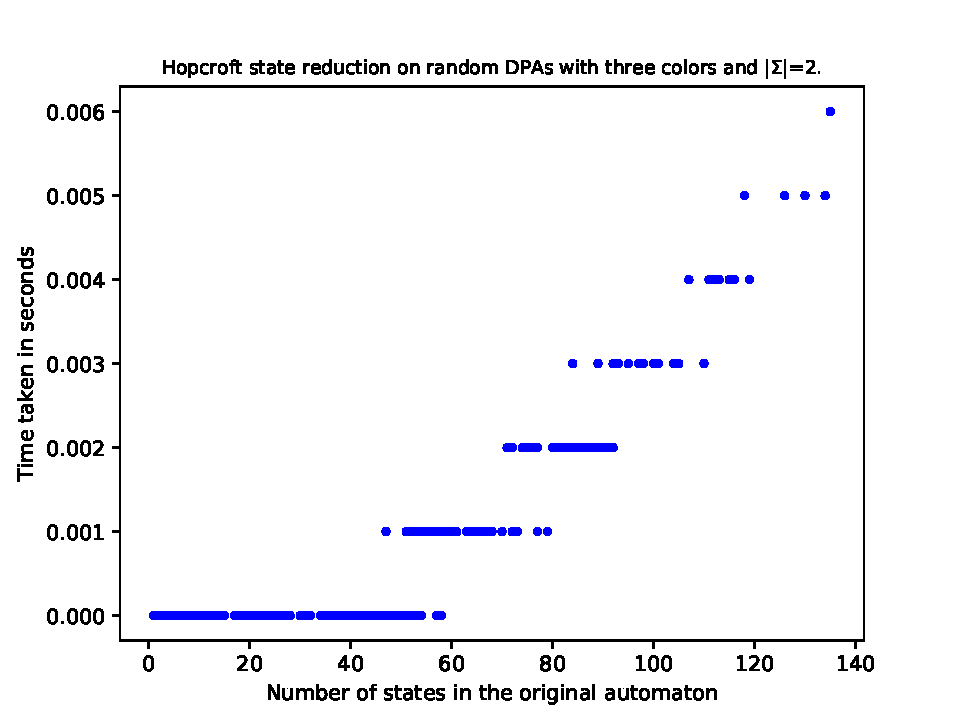
\includegraphics[page=1,height=.3\textheight]{../data/analysis/lsf/gendet_ap1.pdf} 
		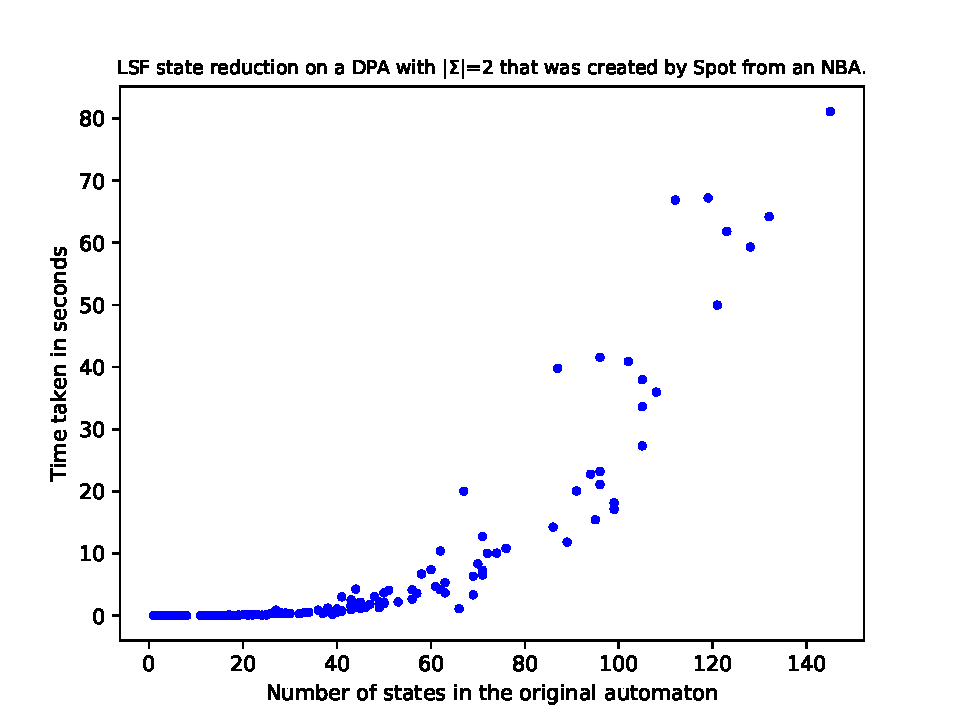
\includegraphics[page=1,height=.3\textheight]{../data/analysis/lsf/detspot_ap1.pdf} 
		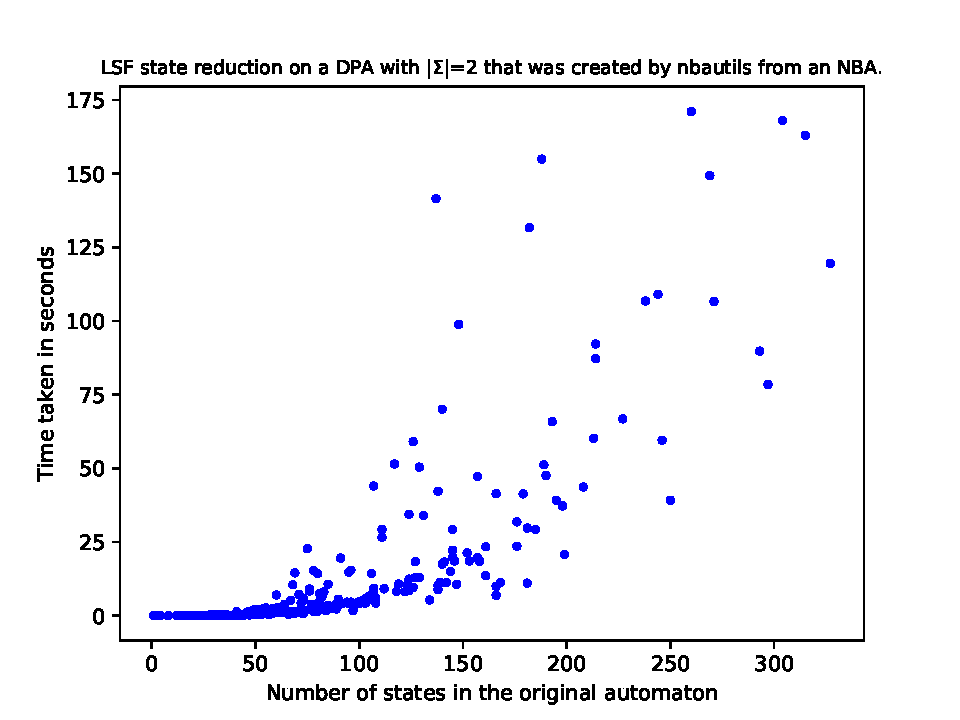
\includegraphics[page=1,height=.3\textheight]{../data/analysis/lsf/detnbaut_ap1.pdf} 
		\caption{Time for state reduction of different automata using $\mu_\text{LSF}^{k,\equiv_L}$.}
		\label{fig:lsf:empirical_time}
	\end{minipage}
\end{figure}

\begin{figure}
	\centering
	\includegraphics[page=6,height=.4\textheight]{../data/analysis/lsf/detnbaut_safra_ap1.pdf} 
	\caption{State reduction of different automata using $\mu_\text{LSF}^{k,\sim}$.}
	\label{fig:lsf:empirical_safra_size_hist}
\end{figure}

\begin{figure}
	\centering
	\includegraphics[page=3,height=.4\textheight]{../data/analysis/lsf/detnbaut_safra_ap1.pdf} 
	\caption{State reduction of different automata using $\mu_\text{LSF}^{k,\sim}$.}
	\label{fig:lsf:empirical_safra_reduct_rel}
\end{figure}

\begin{figure}
	\centering
	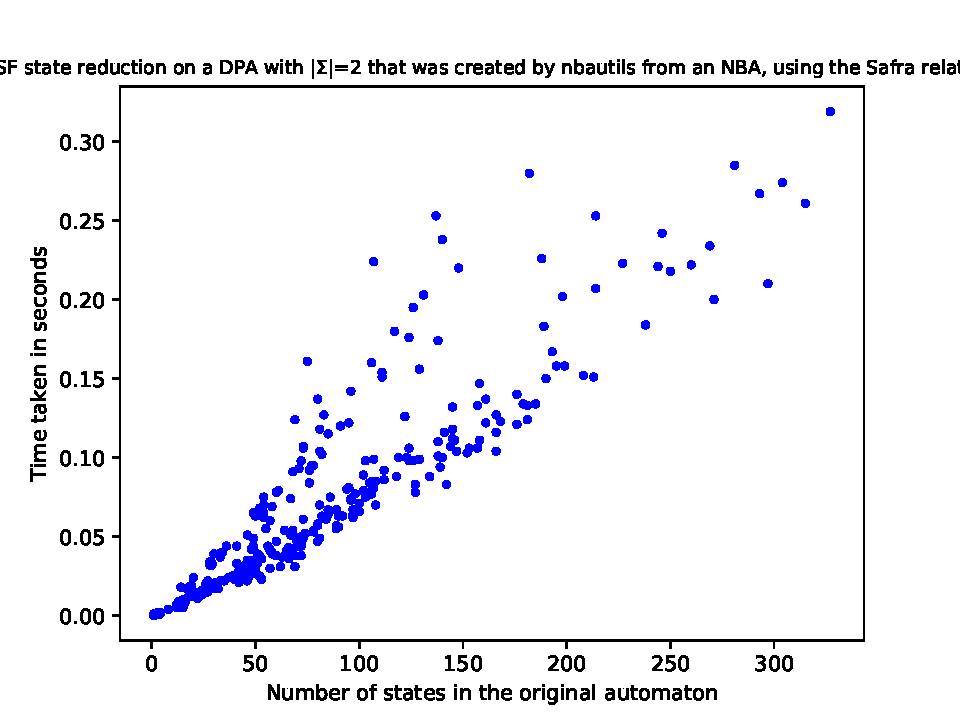
\includegraphics[page=1,height=.4\textheight]{../data/analysis/lsf/detnbaut_safra_ap1.pdf} 
	\caption{State reduction of different automata using $\mu_\text{LSF}^{k,\sim}$.}
	\label{fig:lsf:empirical_safra_time}
\end{figure}


\section{Different Thresholds}

As we did for $\equiv_\text{TM}^\sim$, the question whether we can use a more relaxed relation instead of $\equiv_M^{\leq k}$ arises. For example, we could define $\equiv^{k,\sim}_\text{deLSF}$ to use $\equiv_\text{de}^{\leq k}$ instead and $\mu^{k,\sim}_\text{deLSF}$ analogously. As it turns out, this variant has similar issues as the same approach for $\equiv_\text{TM}^\sim$.

We can use the same example as before, which is again displayed in figure \ref{fig:lsf:desim_counterex1}. The equivalence classes of $\equiv_\text{deLSF}^{1,\equiv_L}$ are $\{ \{q_0, q_2\}, \{q_1\}, \{q_3\} \}$. We can therefore merge $\kappa = \{q_0, q_2\}$ according to the defined rules. In $\mathcal{A} \upharpoonright^c_{> 1}$, $q_0$ and $q_2$ are not connected so we can remove either state and merge it into the other. That means figure \ref{fig:lsf:desim_counterex2} is a representative merge. However, this automaton rejects every word which is not the case for the original.

\begin{figure}
\centering
\begin{tikzpicture}[shorten >=1pt,node distance=2cm,on grid,initial text=]
  \node[state] (0)           	{$q_0$,\{2\}};
  \node[state] (1) [right=of 0] {$q_1$,\{1\}};
  \node[state] (2) [right=of 1] {$q_2$,\{2\}};
  \node[state] (3) [right=of 2] {$q_3$,\{0\}};
  \path[->] (0) edge node [above] {a} (1)
            (1) edge node [above] {a} (2)
            (2) edge [bend left] node [above] {a} (3)
            (3) edge [bend left] node [above] {a} (2);
\end{tikzpicture}
\caption{Example automaton which shows that using $\equiv_\text{de}$ for $\equiv_\text{LSF}$ will not work.}
\label{fig:lsf:desim_counterex1}
\end{figure}

\begin{figure}
\centering
\begin{tikzpicture}[shorten >=1pt,node distance=2cm,on grid,initial text=]
  \node[state] (1)           	{$q_1$,\{1\}};
  \node[state] (0) [right=of 1] {$q_0$,\{2\}};
  \node[state] (3) [right=of 0] {$q_3$,\{0\}};
  \path[->] (0) edge [bend left] node [above] {a} (1)
            (1) edge [bend left] node [above] {a} (0)
            (3) edge node [above] {a} (0);
\end{tikzpicture}
\caption{Example automaton which shows that using $\equiv_\text{de}$ for $\equiv_\text{LSF}$ will not work.}
\label{fig:lsf:desim_counterex2}
\end{figure}













